%\documentclass[10pt, twocolumn]{article}
%\documentclass[11pt]{article}
%\documentclass[twocolumn,showpacs,preprintnumbers,amsmath,amssymb,prl, superscriptaddress]{revtex4}
%\documentclass[twocolumn, preprintnumbers,amsmath,amssymb,prd, superscriptaddress]{revtex4}
\documentclass[preprintnumbers,amsmath,amssymb,prd,superscriptaddress]{revtex4}
%\documentclass[10pt, preprint,showpacs,preprintnumbers,amsmath,amssymb, superscriptaddress]{revtex4}
%\documentclass[11pt, prd,preprintnumbers,amsmath,amssymb, superscriptaddress]{revtex4}
%\documentclass[11pt, prd,preprintnumbers, amsmath,amssymb, superscriptaddress, nofootinbib, hyperref]{revtex4}

\usepackage{latexsym}
\usepackage{amssymb}
\usepackage{epsfig,amsmath,graphics}
\usepackage{epstopdf}
\usepackage{verbatim}
\usepackage{wasysym}
\usepackage{hyperref}
\usepackage{feynmp-auto} % feynman diagrams
%\usepackage{subfig}
\usepackage[utf8]{inputenc}
\usepackage{xpatch}
\usepackage{xcolor}
\usepackage{mathtools}
\hypersetup{
    colorlinks,
    linkcolor={red!80!black},
    citecolor={green!60!black},
    urlcolor={blue!60!black}
}
\usepackage{appendix}

\newcommand{\Ez}{\mathcal{E}_0}
\newcommand{\Eboom}{\mathcal{E}_\text{boom}}
\newcommand{\OO}{\mathcal{O}}
\newcommand{\LL}{\mathcal{L}}
\newcommand{\HH}{\mathcal{H}}
\newcommand{\TeV}{\text{TeV}}
\newcommand{\GeV}{\text{GeV}}
\newcommand{\MeV}{\text{MeV}}
\newcommand{\keV}{\text{keV}}
\newcommand{\rad}{\text{rad}}
\newcommand{\cm}{\text{cm}}
\newcommand{\angstrom}{\buildrel _{\circ} \over {\mathrm{A}}}
\newcommand{\pslash}{p\hspace{-0.070in}/\,}
\newcommand{\Mpl}{M_{\text{pl}}}
\newcommand{\ket}[1]{\ensuremath{\left|#1\right>}}
\newcommand{\bra}[1]{\ensuremath{\left<#1\right|}}
\newcommand{\braket}[2]{\ensuremath{\left<#1|#2\right>}}
%Large Parentheses
\def\r{\right)}
\def\l{\left(}

\begin{document}

%\preprint{APS/123-QED}

\title{Supernovae from Dark Matter Core Collapse in a White Dwarf}

\author{Ryan Janish}
\affiliation{Berkeley Center for Theoretical Physics, Department of Physics,
University of California, Berkeley, CA 94720, USA}

\author{Vijay Narayan}
\affiliation{Berkeley Center for Theoretical Physics, Department of Physics,
University of California, Berkeley, CA 94720, USA}

\author{Paul Riggins}
\affiliation{Berkeley Center for Theoretical Physics, Department of Physics,
University of California, Berkeley, CA 94720, USA}

\begin{abstract}

Dark matter that is capable of sufficiently heating a local region in a white dwarf will trigger runaway fusion and ignite a type 1a supernova.
Here we place further on DM that is captured by white dwarfs, considering the formation and self-gravitational collapse of a DM core.
For asymmetric DM, such a core may form a black hole that ignites a supernovae via Hawking radiation, and for ``almost asymmetric'' DM with non-zero but sufficiently small annihilation cross section may ignite the star via a burst of annihilation during gravitational collapse. 
This extends the constraints from WDs to lower DM masses $m_\chi \gtrsim 10^{7}~\text{GeV}$. 

\end{abstract}

\maketitle


\section{Introduction}
If an energy $\Eboom \sim 10^{16} ~\GeV$ is deposited locally in a white dwarf (WD) within a diffusion time $\tau_\text{diff} \sim 10^{-12}$, it will trigger a type 1a supernova (SN).  
This corresponds to a temperature spike $T_f \sim \MeV$ in a compact region of size $\lambda_T \sim 10^{-5} ~\cm$, and is the necessary condition for runaway fusion, i.e. the rate of carbon fusion trumps the rate of thermal diffusion.
Dark matter (DM) trigger runaway fusion in a WD through the release of high-energy standard model (SM) particles. 
Previously, we have shown this is generally an efficient mechanism for heating the stellar medium regardless of the SM species released.  
Here we focus on the release of particles that occurs during a self-gravitational collapse of a DM core in the star.
If the DM has no self-annihilations (``asymmetric"), then core collapse will result in the formation of a mini black hole (BH).
Such a BH will either evaporate and ignite the WD via Hawking radiation, or accrete and ignite the WD via gravitational heating. 
If the DM has sufficiently small but non-zero annihilation cross section (``almost asymmetric"), then the core collapse may be halted by annihilations.
Such a burst of annihilations can be quite rapid due to the focusing nature of the collapse and is thus capable of igniting the star.

\section{DM Core Collapse}
First we review the physics of DM capture, accumulation, and collapse in a WD in the absence of DM annihilations.
For the remainder of this section all numerical quantities are evaluated at a central WD density $n_\text{ion} \sim 10^{31} ~\cm^{-3}$, for which $M_\text{WD} \approx 1.25 ~M_{\astrosun}$, $R_\text{WD} \approx 4000 ~\text{km}$, and $v_\text{esc} \approx 2 \times 10^{-2}$. 
Depending on the context, the relevant density may be the average value which we take to be $\sim 10^{-1}$ of the central density. 
We also assume a WD temperature $T \sim \text{keV}$, a stellar lifetime $\tau_\text{WD} \sim 5~\text{Gyr}$. 

The transit rate of DM through the star is given by
\begin{align}
  \Gamma_\text{trans} \sim
  \frac{\rho_{\chi}}{m_\chi} \pi R_\text{WD}^2
  \l\frac{v_\text{esc}}{v_\text{halo}}\r^2 v_\text{halo},
\end{align}
where $\rho_\chi$ is the DM density in the region of the WD and $v_\text{halo} \sim 10^{-3}$ is the galactic virial velocity. 
From here on, we take $\rho_\chi \sim 0.4 \GeV/\cm^3$. 
Consider DM with an elastic scattering cross section $\sigma_{\chi A}$ off carbon ions. 
Ultimately we will be interested in DM masses $m_\chi \gg m_\text{ion}$ which result in self-gravitational collapse. 
Here the nuclear momentum transfer is $q \sim m_\text{ion} v_\text{esc} \approx 200 ~\text{MeV}$ and the typical energy transfer per scatter is $\omega \sim m_\text{ion} v_\text{esc}^2 \approx 5 ~\MeV$. 
Since $q$ is of order the inverse nuclear size, the DM-carbon scattering is coherently enhanced.  
The average per-nucleon spin-independent cross section $\sigma_{\chi n}$ is given by
\begin{equation}
\sigma_{\chi A} = A^2 \l \frac{\mu_{A}}{\mu_{n}}\r^2 F^2(q) \sigma_{\chi n} \sim A^4 F^2(q) \sigma_{\chi n},
\end{equation}
where $F^2(q)$ is the Helm form factor. 
At these momentum transfers, we find that $F^2(q) \approx 0.1$.
Currently, the bound on spin-independent DM nuclear elastic scatters is
\begin{equation}
\label{eq:xenon}
\sigma_{\chi n} < 5 \times 10^{-46} ~\text{cm}^2 \l \frac{m_\chi}{10^3 ~\GeV} \r.
\end{equation}
However, bounds from direct detection are only applicable for DM masses less than $\sim 10^{22} ~\GeV$, corresponding to the detector exposure threshold. 
For DM masses greater than this, the bounds are far less stringent. 
During a transit of the WD, the average number of DM scatters is given by
\begin{equation}
N_\text{scat} \sim n_\text{ion} \sigma_{\chi A} R_\text{WD}.
\end{equation}
In general the capture rate of DM is of the form
\begin{align}
  \Gamma_\text{cap} \sim \Gamma_\text{trans} \cdot 
  \text{min}\left\{1, N_\text{scat} \text{min}\{B,1\}\right\}, ~~~~ B \equiv \frac{m_\text{ion} v_\text{esc}^2}{m_\chi v_\text{halo}^2}. 
\end{align}
For $m_\chi > 10 ~\TeV$ and for any scattering cross section satisfying \eqref{eq:xenon}, we see that $\Gamma_\text{cap} < \Gamma_\text{trans}$, and the capture rate scales as $\Gamma_\text{cap} \propto \sigma_{\chi A}/m_\chi^2$.
Of course, the DM velocity will change during its evolution in the star, thus affecting the nature of the DM-carbon scattering. 
For simplicity, in what follows we assume a fixed value of $\sigma_{\chi A}$ valid throughout the range of momentum transfers considered. 

Once DM is captured, it will thermalize in the WD. 
Initially, the DM passes through the WD many times until the size of its orbit is contained in the star.
This takes a time
\begin{align}
  t_1 \sim \l \frac{m_\chi}{m_\text{ion}} \r^{3/2} 
  \frac{R_\text{WD}}{v_\text{esc}} \frac{1}{N_\text{scat}} 
  \frac{1}{\text{max}\{N_\text{scat}, 1\}^{1/2}} 
  \approx 2 \times 10^{9}~\text{s} \l \frac{m_\chi}{10^{10} ~\GeV} \r^{3/2} 
  \l \frac{\sigma_{\chi A}}{10^{-36} ~\cm^2} \r^{-3/2}.
\end{align}
This stage is relevant only if the energy loss after a single transit does not exceed $\sim m_\chi v_\text{esc}^2$:
\begin{equation}
\l \frac{m_\text{ion}}{m_\chi} \r \text{max}\{\bar{N}_\text{scat},1\} < 1,
\end{equation}
which is the case for any cross section which satisfies \eqref{eq:xenon}. 
Subsequently, the DM orbital size decays until it is order the thermal radius. 
This takes a time
\begin{align}
 t_2 \sim \l \frac{m_\chi}{m_\text{ion}} \r \frac{1}{n_\text{ion} \sigma_{\chi A}} \frac{1}{v_\text{ion}} \left \{ 1+\log \l \frac{m_\chi}{m_\text{ion}}\r \right \}
  \approx 10^9 ~\text{s} \l \frac{m_\chi}{10^{10} ~\GeV} \r \l \frac{\sigma_{\chi A}}{10^{-36} ~\cm^2} \r^{-1}.
\end{align}
Note the additional logarithmic factor once the DM velocity drops below $v_\text{ion} \sim \sqrt{\frac{T}{m_\text{ion}}}$. 
By far the shortest timescale is the dynamical free-fall time:
\begin{equation}
\label{eq:freefalltime}
t_\text{ff} \sim \sqrt{\frac{1}{G \rho_\text{WD}}} \approx 0.5 ~\text{s}.
\end{equation}

Assuming that $t_1 + t_2 < \tau_\text{WD}$, DM will begin steadily accumulating at the thermal radius where its kinetic energy balances against the gravitational potential energy of the enclosed WD mass:
\begin{align}
  R_\text{th} \sim v_\text{th} t_\text{ff} \approx 50 ~\cm \l \frac{m_\chi}{10^{10} ~\GeV}\r^{-1/2}, ~~~~   v_\text{th} \sim \sqrt{\frac{T}{m_\chi}} \approx 10^{-8} \l \frac{m_\chi}{10^{10} ~\GeV}\r^{-1/2}.
\end{align}
The maximum number of DM particles that the WD can accumulate is
\begin{align}
N_\text{life}  \sim \Gamma_\text{cap} \tau_\text{WD} \approx 10^{31}  \l \frac{m_\chi}{10^{10} ~\GeV} \r^{-2}  \l \frac{\sigma_{\chi A}}{10^{-36} ~\cm^2} \r.
\end{align}
However, if the DM density at the thermal radius ever exceeds the WD density, then self-gravitational collapse will kick in. 
The critical number of DM particles needed for self-gravitation is
\begin{align}
\label{eq:Nsg}
    N_\text{sg} \sim \frac{\rho_\text{WD} R^3_\text{th}}{m_\chi} \approx 2 \times 10^{27} \l \frac{m_\chi}{10^{10} ~\GeV} \r^{-5/2}.
\end{align}
Thus if there are no annihilations, the condition for a collapse is simply $N_\text{sg} < N_\text{life}$.
This sets a lower bound on DM mass---if the scattering cross secion is saturated at its largest allowed value \eqref{eq:xenon}, collapse requires $m_\chi \gtrsim 10^{7} ~\GeV$. 
Note that the DM population at $R_\text{th}$ prior to collapse is adequately described by Maxwell-Boltzmann statistics if $N_\text{sg}$ is less than $R_\text{th}^3 (m_\chi T)^{3/2} \approx 10^{52}$, which is clearly true in this case. 

Now we turn to the dynamics of DM collapse for a number of collapsing particles $N_\text{sg}$. 
In order for the DM sphere to shrink, it must shed the excess gravitational potential energy. 
If the only source of dissipation is elastic nuclear scatters, the ``cooling" timescale is initially independent of DM velocity $v_\chi$ but hastens once the DM velocity exceeds $v_\text{ion}$: 
\begin{equation}
\label{eq:tcool}
t_\text{cool} \sim \frac{m_\chi}{\rho_\text{WD} \sigma_{\chi A}} \frac{1}{\text{max}\{{v_\text{ion},v_\chi\}}}.
\end{equation}
As the cooling time is far greater than the virialization time, DM particles in the collapsing sphere will have velocity $v_\chi \sim \sqrt{\frac{G N_\text{sg} m_\chi}{r}}$, where $r$ denotes the size of the DM sphere. 
Of course, the density of the collapsing DM will not be entirely uniform.
More likely, the DM will establish a density profile similar to galactic halos that is somewhat cuspy. 
For simplicity, we will assume a uniform density throughout the collapse---this is certainly possible if there are substantial DM-DM elastic scatters. 

As the DM sphere shrinks, there may be some stabilizing pressure or repulsive self-interaction which prevents collapse below a certain radius.
Famously, gravity itself provides such a ``pressure", arresting collapses below the Schwarzschild radius by the formation of a black hole (BH) 
\begin{equation}
R_\text{BH} \sim G N_\text{sg} m_\chi \approx 5 \times 10^{-15} ~\cm \l \frac{m_\chi}{10^{10} ~\GeV} \r^{-3/2}.
\end{equation}
There may be some pressure due to quantum statistics.
The quantum nature of DM becomes relevant once the de Broglie wavelength of individual DM particles $\sim \frac{1}{m_\chi v_\chi}$ exceeds their physical separation $\sim \frac{r}{N_\text{sg}^{1/3}}$:
\begin{equation}
\label{eq:deg}
R_\text{QM} \sim \frac{1}{G m_\chi^3 N_\text{sg}^{1/3}} \approx 10^{-15} ~\cm \l\frac{m_\chi}{10^{10} ~\GeV}\r^{-13/6}.
\end{equation}
This occurs before the formation of a BH for DM masses
\begin{equation}
\label{eq:qm}
m_\chi < \frac{\rho_\text{WD}}{T^3} \approx 10^{9} ~\GeV.
\end{equation}
We treat fermion DM and boson DM separately below. 

\textcolor{red}{clarify}
We briefly mention a subtlety that arises in the DM core collapse for sufficiently large $m_\chi$. 
The time to collect a self-gravitating number of particles $t_\text{sg} = N_\text{sg}/\Gamma_\text{cap} \propto m_\chi^{-1/2}$ decreases for larger DM masses. 
However, the dynamics of the collapse is set by the cooling time, which is initially $t_\text{cool} \propto m_\chi$. 
We find that for $m_\chi > 10^{14} ~\GeV$, the collection time is shorter than the cooling time $t_\text{sg} < t_\text{cool}$.
In fact, the collection time may even be shorter than the dynamical time $t_\text{ff}$.
This is the case for $m_\chi > 10^{19} ~\GeV$. 
We consider the following scenarios: 
If $t_\text{ff} < t_\text{sg} <t_\text{cool}$, the DM core will be driven to shrink because of the gravitational potential of the overcollecting DM.
The timescale for the shrinking is set by the capture rate of DM. 
Ultimately, the collapsing DM core will consist of $N_\text{sg}$ enveloped in a ``halo" of $N \gg N_\text{sg}$ particles. 
If $t_\text{sg} < t_\text{ff} <t_\text{cool}$, the DM core will rapidly accumulate particles before dynamically adjusting.
Thus the number of collapsing particles is much larger than $N_\text{sg}$
Note that the number of DM particles needed for self-gravitation $N_\text{sg}$ should properly saturate to a minimum of two---this takes place when $m_\chi > 10^{21} ~\GeV$. 

\subsection{Fermion DM}
If the DM is a fermion, $R_\text{QM}$ is precisely the radius of stabilization due to degeneracy pressure.
In this case, the degenerate DM core at $R_\text{QM}$ will continue to collect DM (and shrink accordingly) until it reaches the Chandrasekhar number
\begin{equation}
N^\text{f}_\text{Cha} \sim \frac{1}{G^{3/2} m_\chi^3} \approx 10^{33} \l \frac{m_\chi}{10^{8} ~\GeV}\r^{-3},
\end{equation}
at which point it collapses to a BH. 
Note that additional captured DM particles are still able to dissipate energy and decrease their orbital size below the thermal radius under the gravitational influence of the compact core. 
Thus the degenerate core accretes DM at a rate $\Gamma_\text{cap}$ and eventually forms a BH as long as $N^\text{f}_\text{Cha} < N_\text{life}$. 

\subsection{Boson DM}
If the DM is a boson, the dynamics of the collapse are slightly more involved.
The pressure induced by the uncertainty principle is insufficient to prevent collapse of a self-gravitating sphere of DM particles if the number exceeds the
 ``bosonic" Chandrasekhar number
\begin{equation}
\label{eq:boscha}
N^\text{b}_\text{Cha} \sim \frac{1}{G m_\chi^2} \approx 10^{22}  \l \frac{m_\chi}{10^{8} ~\GeV}\r^{-2}.
\end{equation}
This is far less than $N_\text{sg}$. 
However, once the DM sphere reaches $R_\text{QM}$, it will begin populating a Bose Einstein condensate (BEC) at the center.
Here the density of the DM sphere is of order
\begin{equation}
\rho_\text{crit} \sim \frac{m_\chi^5 T^3}{\rho_\text{WD}}.
\end{equation}
Note that a BEC forms on a timescale much shorter than any other.
Further collapse of the DM sphere results in increasing the number of particles in the condensate while the density of the non-condensed particles remains fixed at $\rho_\text{crit}$. 
The size of the BEC is set by the gravitational potential of the self-gravitating sphere
\begin{equation}
R_\text{BEC} \sim \l \frac{1}{G \rho_\text{crit} m_\chi^2}\r^{1/4} \approx 10^{-16} ~\cm \l \frac{m_\chi}{10^{8} ~\GeV} \r^{-7/4}.
\end{equation}
Particles in the BEC remain at $R_\text{BEC}$ and have velocity $v_\text{BEC} \sim \frac{1}{m_\chi R_\text{BEC}}$ until the condensate itself has enough particles to become self-gravitating: 
\begin{equation}
N^\text{sg}_\text{BEC} \sim \frac{\rho_\text{crit} R_\text{BEC}^3}{m_\chi} \approx 10^{16} \l \frac{m_\chi}{10^{8} ~\GeV} \r^{-5/4},
\end{equation}
Thus, the condensate will continue to accumulate particles until it reaches $N^\text{b}_\text{Cha}$. 
During this time the BEC is shrinking in size as $\sim \frac{1}{G m_\chi^3 N_\text{BEC}}$.
The rate at which DM particles are added to the BEC is set by the rate at which the non-condensed DM sphere sheds the excess gravitational energy.
If the DM sphere is initially at $R_\text{QM}$ and has $N_\text{sg}$ particles it must lose an energy $\sim \frac{G N_\text{sg} N_\text{BEC} m_\chi^2}{R_\text{QM}}$ in order to add $N_\text{BEC} \ll N_\text{sg}$ particles to the condensate. 
The timescale for this is
\begin{equation}
\label{eq:tbec}
t^\text{cool}_\text{BEC} \sim \frac{N_\text{BEC}}{\rho_\text{WD} \sigma_{\chi A}v_\chi^3} \frac{G N_\text{sg} m_\chi^2}{R_\text{QM}} \approx 10^{-9} ~\text{s} \l \frac{N_\text{BEC}}{N^\text{b}_\text{Cha}} \r \l \frac{m_\chi}{10^{8} ~\GeV} \r^{7/6} \l \frac{\sigma_{\chi A}}{10^{-36} ~\cm^2} \r^{-1}.
\end{equation}
Note the velocities of non-condensed DM particles are nearly relativistic at this stage $v_\chi \sim \sqrt{\frac{G N_\text{sg} m_\chi}{R_\text{QM}}} \gtrsim 0.1$. 
After a time $t^\text{cool}_\text{BEC}$, a BH is born within the DM sphere. 

\section{Black Holes and Asymmetric DM}
We have outlined above the conditions such that core collapse of asymmetric DM in a WD leads to formation of a BH. 
For sufficiently heavy DM quantum statistics is never relevant during the collapse and resulting BH mass is:
\begin{equation}
M_\text{BH} = N_\text{sg} m_\chi \approx 2 \times 10^{37} ~\GeV \l \frac{m_\chi}{10^{10} ~\GeV} \r^{-3/2}.
\end{equation} 
For DM masses satisfying \eqref{eq:qm}, if the DM is a fermion then
\begin{equation}
M_\text{BH} = N^\text{f}_\text{Cha} m_\chi \approx 10^{41} ~\GeV \l \frac{m_\chi}{10^{8} ~\GeV} \r^{-2},
\end{equation} 
while if the DM is a boson then
\begin{equation}
\label{eq:BHboson}
M_\text{BH} = N^\text{b}_\text{Cha} m_\chi \approx 10^{30} ~\GeV \l \frac{m_\chi}{10^{8} ~\GeV} \r^{-1}.
\end{equation} 

First we discuss the fate of newly formed BHs of mass $M$. 
As shown by Hawking, BHs have a temperature $T_\text{BH} \sim \frac{1}{G M}$ and predominantly radiate SM particles of mass less than $T_\text{BH}$. 
The rate of BH evaporation due to Hawking radiation is
\begin{equation}
\dot{M}_\text{HR} = \frac{\alpha}{G^2 M^2},
\end{equation}
where $\alpha(M)$ characterizes the thermal spectrum emitted at a given BH mass.
Naive dimensional analysis yields $\alpha = \frac{1}{15360 \pi}$. 
Detailed numerical analysis find $\alpha \approx 2 \times 10^{-4}$ for $T_\text{BH} \lesssim \MeV$ while $\alpha \approx 4 \times 10^{-3}$ for $T_\text{BH} \gtrsim 100 ~\GeV$. 
In the absence of any accretion, a BH will evaporate within the age of the WD if
\begin{equation}
\label{eq:HRlife}
M < \l \frac{3 \alpha \tau_\text{WD}}{G^2}\r^{1/3} \approx 2 \times 10^{38} ~\GeV~~~~ (\text{evaporate in WD lifetime}). 
\end{equation}

There are two primary sources of accretion onto the BH.
The Bondi accretion of nuclear matter is of the form
\begin{equation}
\dot{M}_\text{Bondi} = \beta \rho_\text{WD} G^2 M^2,
\end{equation}    
where $\beta$ is a coefficient of order $\beta \sim 4 \pi/c_s^3 \approx 10^7$. 
There is also the accretion of additional DM particles.
If a particle crosses the radius of efficient BH accretion $4GM$, it will rapidly fall into the BH. 
Once the BH is formed individual DM particles are still ``cooling" via elastic nuclear scatters, reducing their orbital sizes below the thermal radius. 
In steady state, the rate at which DM orbits reach this threshold is given by the DM capture rate $\Gamma_\text{cap}$. 
Thus the accretion rate due to DM is 
\begin{equation}
\dot{M}_\text{DM} = \Gamma_\text{cap} m_\chi. 
\end{equation}
We see that $\dot{M}_\text{HR}$ is greater than $\dot{M}_\text{Bondi}$ for BH masses
\begin{equation}
\label{eq:beatbondi}
M < \l \frac{\alpha}{\beta \rho_\text{WD}}\r^{1/4} \frac{1}{G} \approx 4 \times 10^{37} ~\GeV ~~~~ (\text{Hawking beats Bondi}).
\end{equation}
We have checked that the Bondi accretion is not Eddington-limited at $M \approx 4 \times 10^{37} ~\GeV$. 
Similarly, $\dot{M}_\text{HR}$ is greater than $\dot{M}_\text{DM}$ for BH masses
\begin{equation}
\label{eq:beatDM}
M < \l \frac{\alpha}{\Gamma_\text{cap} m_\chi}\r^{1/2} \frac{1}{G} \approx 3 \times 10^{36} ~\GeV \l \frac{m_\chi}{10^{10} ~\GeV} \r^{1/2} \l \frac{\sigma_{\chi A}}{10^{-36} ~\cm^2} \r^{-1/2}~~~~ \text{(Hawking beats DM}). 
\end{equation}

However, if a BH is formed via a self-gravitating BEC within a non-condensed DM sphere, the DM accretion rate is actually much larger due to the density $\rho_\text{crit} \gg \rho_\text{WD}$ of the surrounding DM sphere.
Here the rate of DM accretion is given by the spherical, collisionless approximation:
\begin{equation}
\dot{M}_\text{DM} = \frac{16 \pi \rho_\text{crit} G^2 M^2}{v_\chi},
\end{equation}
where $v_\chi \sim \sqrt{\frac{G N_\text{sg} m_\chi}{R_\text{QM}}}$ is typical velocity of DM far away from the BH. 
We have checked that for such a BH with mass \eqref{eq:BHboson}, the rate of DM accretion is larger than the rate of evaporation. 
In this case, the characteristic accretion timescale $\tau_\text{acc} \sim M/\dot{M}$ is of order
\begin{equation}
\tau_\text{acc} \sim \frac{v_\chi}{16 \pi \rho_\text{crit} M_\text{BH} G^2} \approx 6 \times 10^{-12} ~\text{s} \l \frac{m_\chi}{10^{8} ~\GeV} \r^{-11/3}.
\end{equation}
Note that this timescale is always shorter than the timescale \eqref{eq:tbec} to condense a new BH. 

We now show that any BH formed in the WD will inevitably trigger a SN during the course of its evolution. 
If the BH is evaporating, it will ignite the star once the mass is sufficiently small that it releases an energy $\Eboom$ via Hawking radiation within a time $\tau_\text{diff}$:
\begin{equation}
M < \l \frac{\alpha \tau_\text{diff}}{\Eboom}\r^{1/2} \frac{1}{G} \approx 10^{34} ~\GeV ~~~~ (\text{boom from Hawking radiation}).
\end{equation}
Note that any evaporating BH satisfying \eqref{eq:beatbondi} and \eqref{eq:beatDM} also satisfies \eqref{eq:HRlife}, and will thus necessarily reach this mass within $\tau_\text{WD}$. 
Hawking radiation can even ignite the star if the BH is accreting but is initially very small. 
This is the case for BHs that originate from a BEC and are accreting due to DM capture.
It can be shown that such BHs release enough energy before having a chance to substantially grow in size:
\begin{equation}
\frac{\alpha}{G^2 M_\text{BH}^2} \text{min}\{\tau_\text{acc},\tau_\text{diff}\} > \Eboom.
\end{equation}
If the BH is accreting and violates either \eqref{eq:beatbondi} or \eqref{eq:beatDM}, it will still ignite the star. 
This occurs once the mass is sufficiently large that it gravitationally accelerates carbon ions within a distance $\lambda_T$ to energies $T_f \sim \MeV$:
\begin{equation}
M > \l \frac{T_f}{m_\text{ion}} \r \frac{\lambda_T}{G} \approx 10^{43} ~\GeV ~~~~ (\text{boom from gravitational heating}). 
\end{equation}
In such cases, the accretion timescale is always shorter than $\tau_\text{WD}$ even if Bondi accretion is Eddington-limited at higher BH masses. 
Note that the BH radius is less than $\lambda_T$ for $M < 10^{46} ~\GeV$, while the BH evaporation time is longer than $\tau_\text{diff}$ for $M > 4 \times 10^{28} ~\GeV$.

Thus, we can constrain any model of heavy, asymmetric DM which collapses to a BH based on the observation of several heavy, long-lived WDs. 
This is done in Figures \ref{fig:BHfermion} and \ref{fig:BHboson} for fermion and boson DM, respectively. 

\begin{figure}
\centering
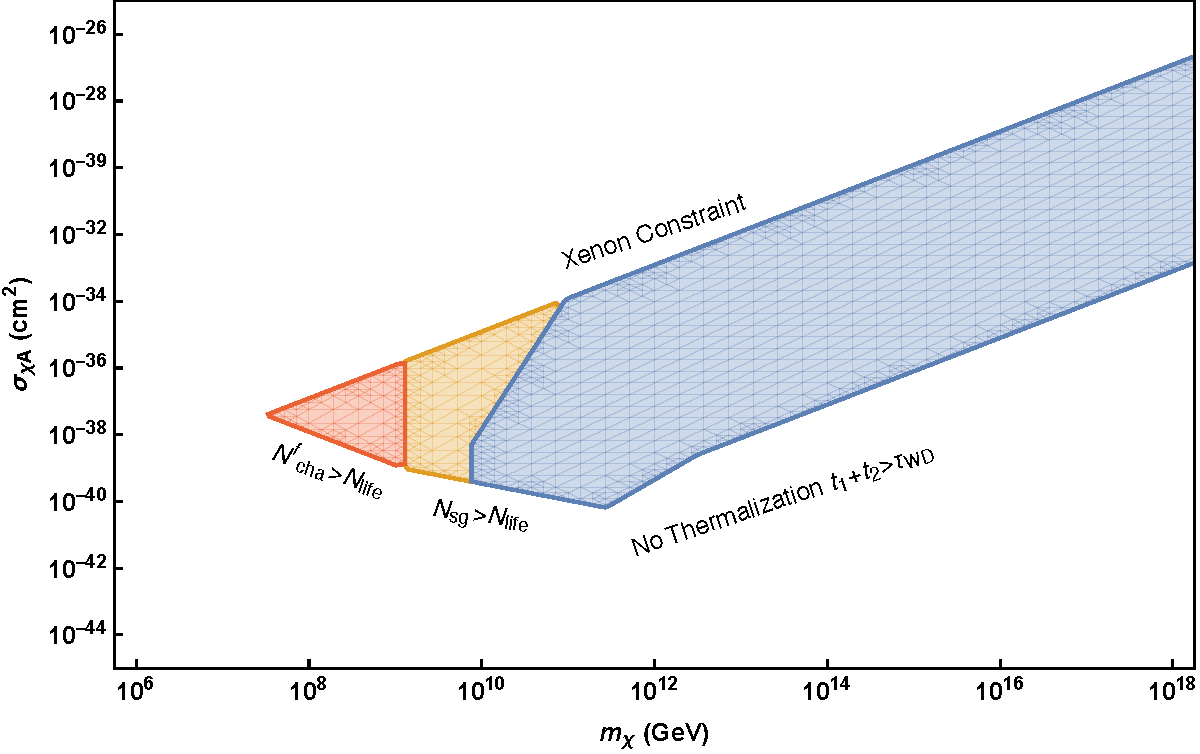
\includegraphics[scale=0.5]{BHfermion}
\caption{Constraints on fermion asymmetric DM through core collapse and BH formation in a WD.
BH of initial mass $M_\text{BH} = N_\text{sg} m_\chi$ will ignite a SN within WD lifetime via Hawking radiation (blue) or gravitational heating (orange).
If the collapse is stabilized by degeneracy pressure, it will ultimately result in a BH of initial mass $M_\text{BH} = N^\text{f}_\text{Cha} m_\chi$ that ignites SN via gravitational heating (red).
}
\label{fig:BHfermion}
\end{figure}

\begin{figure}
\centering
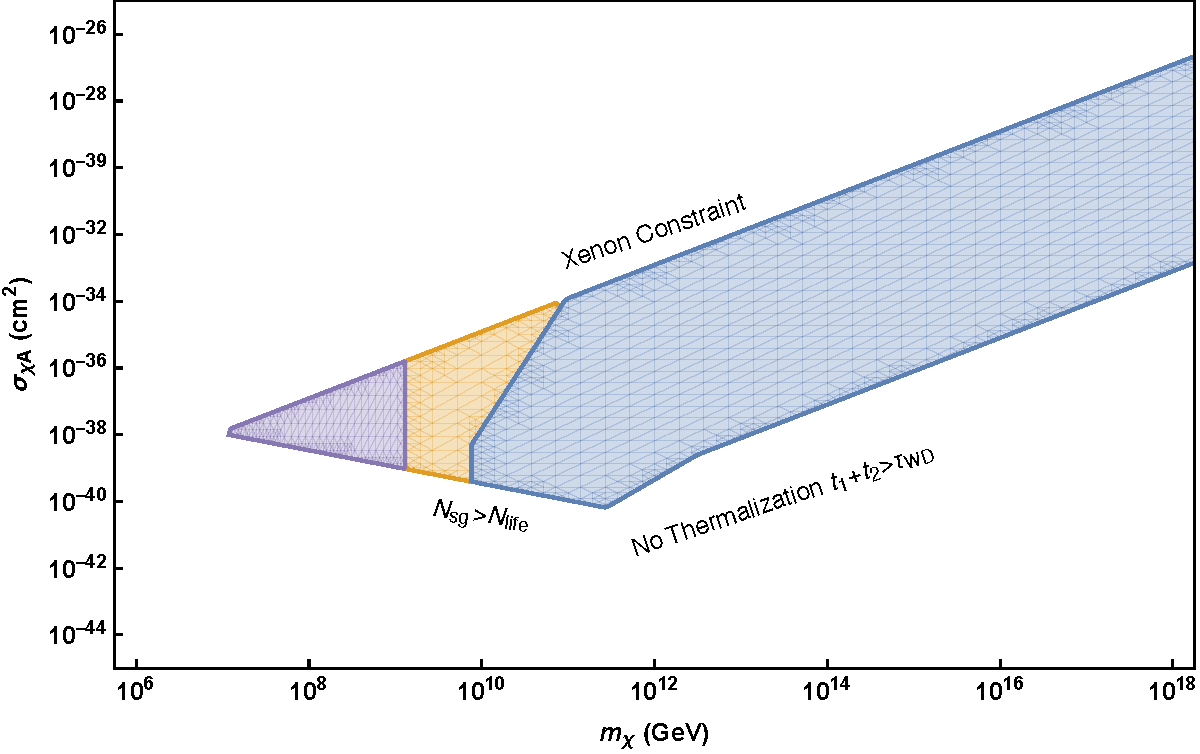
\includegraphics[scale=0.5]{BHboson}
\caption{Constraints on boson asymmetric DM through core collapse and BH formation in a WD.
BH of initial mass $M_\text{BH} = N_\text{sg} m_\chi$ will ignite a SN within WD lifetime via Hawking radiation (blue) or gravitational heating (orange).
If a BEC is populated, it will ultimately result in a BH of initial mass $M_\text{BH} = N^\text{b}_\text{Cha} m_\chi$ that ignites SN via Hawking radiation (purple).}
\label{fig:BHboson}
\end{figure}

\section{Core Collapse with DM Annihilations}

Suppose the DM has an annihilation cross section $\sigma_{\chi \chi}$ into SM particles.
Here we assume that $m_\chi < \Eboom$, so that a single annihilation is unable to trigger a SN. 
However, under certain conditions the sum total of multiple annihilations during DM core collapse will be able to ignite the star. 

First we examine the effect of annihilations on the physics of DM capture, accumulation, and collapse. 
To begin, the thermalizing DM constitutes a number density of DM throughout the WD volume as well as outside the star. 
The total rate of annihilations for this DM population is dominated near the thermal radius:
\begin{equation}
\Gamma_\text{infall} \sim \frac{(\Gamma_\text{cap} t_2)^2}{R_\text{th}^3} \sigma_{\chi \chi} v_\text{th}. 
\end{equation}
Depletion of the thermalizing DM is negligible if
\begin{equation}
\label{eq:steadycollect}
\Gamma_\text{infall} < \Gamma_\text{cap},
\end{equation}
in which case the rate of DM accumulation at $R_\text{th}$ is roughly given by the rate of capture $\Gamma_\text{cap}$. 
Of course, this density of accumulating DM is also depleting due to annihilations. 
Once the DM annihilation rate at the thermal radius is of order the DM capture rate, the number of DM particles saturates to:
\begin{align}
N_\text{sat} \sim \l \frac{\Gamma_\text{cap} R_\text{th}^3}{\sigma_{\chi \chi} v_\text{th}} \r^{1/2} \approx 5 \times 10^{30} \l \frac{m_\chi}{10^{10} ~\GeV} \r^{-3/2} \l \frac{\sigma_{\chi \chi}}{10^{-45} ~\cm^2} \r^{-1/2}  \l \frac{\sigma_{\chi A}}{10^{-36} ~\cm^2} \r^{1/2}.
\end{align}
Thus in the presence of annihilations, the condition for collapse becomes modified:
\begin{equation}
\label{eq:collapsecond}
N_\text{sg} < \text{min}\{N_\text{life}, N_\text{sat}\}.
\end{equation}
There are two potential evolutions of the captured DM: either the DM collapses or it does not. 
In the later case, the DM has either reached its saturation number at the thermal radius or is still continuing to accumulate, not yet having the critical number necessary for collapse in its lifetime.
This scenario does not yield any constraints on DM parameters which ignite the star:
\begin{equation}
\label{eq:nocollapse}
m_\chi \l \frac{\text{min}\{N_\text{eq}, N_\text{life}\}}{R_\text{th}^3}\r^2 \sigma_{\chi \chi} v_\text{th} \lambda_T^3 \tau_\text{diff} \ll \Eboom, ~~~~ N_\text{sg}>\text{min}\{N_\text{eq}, N_\text{life}\}.
\end{equation}

Thus we turn our attention to DM core collapse.
Here, the dynamics of the collapse differs from the asymmetric case in that the number of collapsing particles is depleting due to annihilations. 
If the DM sphere consisting of $N_\text{sg}$ particles is at a radius $r$, the characteristic timescale for annihilations is:
\begin{equation}
t_\text{ann} \sim \frac{r^3}{N_\text{sg} \sigma_{\chi \chi} v_\chi}, ~~~~ v_\chi \sim \sqrt{\frac{G N_\text{sg} m_\chi}{r}}.
\end{equation}
As before, the DM sphere shrinks at a timescale set by cooling \eqref{eq:tcool} 
Thus, the collapse of the entire DM sphere proceeds roughly unscathed until $t_\text{ann} \sim t_\text{cool}$, at which point annihilations become relevant and the number of collapsing particles is depleting by $\OO(1)$.
The radius of the DM sphere at which the annihilation and cooling timescales match is an important scale which we denote as $R_{\chi \chi}$:
\begin{equation}
R_{\chi \chi} =  \text{min}\{R_1, R_2\},
\end{equation}
where 
\begin{align}
R_1 \sim R_\text{th} \l \frac{\sigma_{\chi \chi}}{\sigma_{\chi A}}\r^{2/7} \l \frac{m_\text{ion}}{m_\chi} \r^{1/7}, ~~~~ R_2 \sim R_\text{th} \l \frac{\sigma_{\chi \chi}}{\sigma_{\chi A}}\r^{1/3}. 
\end{align}
distinguishes between the two different expressions for $t_\text{cool}$ based on the DM velocity. 
Of course such a collapse is only sensible if
\begin{align}
\label{eq:xicondition}
R_{\chi \chi} < R_\text{th},
\end{align}
which is trivially satisfied assuming both \eqref{eq:steadycollect} and \eqref{eq:collapsecond} are satisfied.

When the DM core is at a radius $r$, the energy released via annihilations is sufficient to trigger a SN if
\begin{equation}
\label{eq:annburst}
E_\text{ann} \sim m_\chi \l \frac{N_\text{sg}}{r^3}\r^2 \sigma_{\chi \chi} v_\chi \text{min}\{r,\lambda_T\}^3 \tau_\text{diff} > \Eboom.
\end{equation}
As expected, the rate of energy injection increases as the size of the DM core shrinks. 
However, there is a minimum size $R_{\chi \chi}$ beyond which annihilations efficiently deplete the collapsing core.
Replacing $r \to R_{\chi \chi}$ in $E_\text{ann}$, we find that the DM core is in fact more explosive for low annihilation cross section and low DM mass. 
For instance, for $R_{\chi \chi} <\lambda_T$, the energy released scales as $E_\text{ann} \propto m_\chi^{-2} \sigma_{\chi \chi}^{-1/6}$.

However, BH formation or the onset of degeneracy pressure may halt the collapse before $R_{\chi \chi}$. 
For fermion DM, $E_\text{ann}$ is maximized by taking $r \sim \text{max}\left \{R_{\chi \chi}, \text{max}\{R_\text{BH}, R_\text{QM}\} \right \}$. 
In the case that the DM core reaches $R_\text{QM}$ and is stabilized by degeneracy pressure before depleting, it will continue to accumulate particles and shrink---we have checked that the energy released via annihilations during this process is not sufficient to ignite the star. 
For boson DM, the DM sphere collapses at fixed density $\rho_\text{crit}$ upon reaching $R_\text{QM}$. 
Here the rate of energy injection decreases as the size of the non-condensed DM core shrinks, so again $E_\text{ann}$ is maximized by taking $r \sim \text{max}\left \{R_{\chi \chi}, \text{max}\{R_\text{BH}, R_\text{QM}\} \right \}$.
We may also examine annihilations of the BEC both before and after self-gravitation---this constrains even lower annihilation cross sections.

We can constrain any model of ``almost asymmetric" DM which annihilates and ignites a SN during core collapse.
Only those scattering cross sections $\sigma_{\chi A}$ satisfying the conditions for collapse (e.g. $t_1 +t_2 <\tau_\text{WD}$) can be constrained. 
On the other hand, the constraints extend to extremely annihilation cross section $\sigma_{\chi \chi}$.
Constraints on such DM are shown in Figure \ref{fig:annbur} for a benchmark value of $\sigma_{\chi A} = 10^{36}$---this corresponds to scattering via Z-exchange. 
An explicit model of DM with such an interaction is asymmetric, hyper-charged DM with a tiny Majorana mass term. 
More generally, any asymmetric DM which can annihilate itself through higher-dimension operators. 

\begin{figure}
\centering
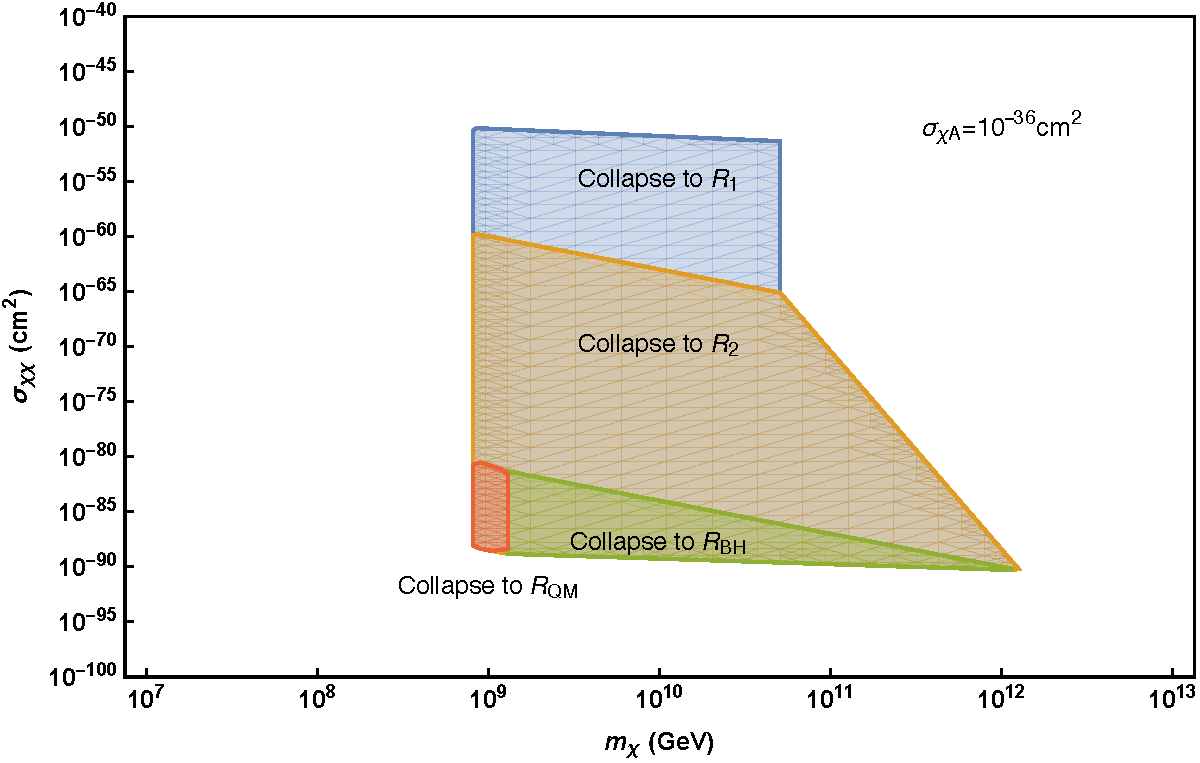
\includegraphics[scale=0.5]{annbur}
\caption{Constraints on DM annihilation during core collapse in a WD.
The collapse is either halted at $R_{\chi \chi}$---$R_1$ (blue), $R_2$ (orange)---or $R_\text{BH}$ (green).
If DM is a fermion, collapse is halted by degeneracy pressure at $R_\text{QM}$. 
If DM is a boson, collapse proceeds at constant density at $R_\text{QM}$ due to BEC formation.
Both scenarios yield the same constraints (red).}
\label{fig:annbur}
\end{figure}

\section{Discussion}

\end{document}